\documentclass[11pt]{article}

\usepackage[letterpaper, margin=1cm]{geometry}
\usepackage{hyperref}
\usepackage{graphicx}
\graphicspath{ {./images/} }
\usepackage{wrapfig}    % For wrapping text around figures
\usepackage{caption} 
\usepackage{float}
%\usepackage{amsmath}
%\usepackage{amssymb}
\usepackage{listings}

\title{Shadow Spy\\Introduction to Computer Graphics (COS426)}
\author{Simon Sure (ss9971@princeton.edu / simon.sure@inf.ethz.ch)\\
        Flurin Steck (fs7278@princeton.edu / flurin.steck@inf.ethz.ch)}

\begin{document}
\maketitle
\textit{Shadow Spy} is a two-player hide-and-seek game. Each player navigates a dark shared world from his own first-person perspective, carrying a flashlight. A player wins by finding their opponent and observing him them sufficiently long first. Players can choose between different scenes.
\par The game is implemented with \texttt{three.js}, decentralized WebRTC based browser-to-browser communication, and Blender 3D models with animations. We make extensive use of libraries for audio, ray casting and other features, and custom implementations for collision detection and handling, first-person controls, and more.

%\tableofcontents




% -----------------------------------------------------------------

\section{Goals}
\par Looking at previous projects, we decided to bring a new and unique feature to our game. We decided to make a multi-player game, which influenced all subsequent design decisions.
\par The idea for the gameplay was quickly developed. The \textit{Results} section elaborates extensively how the game works. We discuss more specific goals in this section.

\subsection{Networking}
\par Implementing a multi-device multiplayer game requires networked communication between the players. Most games use a centralized setup. To (a) not having to operate the server infrastructure and (b) not having to develop a separate server backend, we wanted to utilize direct browser-to-browser communication. This technology has been advanced in recent years, mostly as part of WebRTC.
\par Our plans for a multi-player game would require synchronization. Because the goal was to randomize the scenes, we couldn't only load static resources. During the game, the player movements would have to be synchronized at a sufficient rate for an interactive gameplay.
\par Using direct browser-to-browser communication generally provides lower latency than a centralized approach. This makes the game even more interactive. When both players are physically close, the latency is practically unnoticeable.

\subsection{Graphics Software}
\par We knew from the beginning that our game would require a lot of functionality to support a smooth user experience. We would have to implement first-person controls, use ray-casting to detect when one views another user, perform collision detection, support for multiple scenes, support for networking, ... Thus we put a focus on a modular high-level software architecture for our project.

\subsection{Functionality}
\par Our initial ideas for additional features went far beyond what we had time to implement. We discussed adding weather, placing power-up items in the world, … Given careful planing of the software architecture, those features would be reasonable to implement with a considerable time investment.
\par Considering the time limitation, we created a list of essential features for the game to be usable and focussed on implementing those quickly. Afterward, we could add features as time allows.
\par The essential features were: First-person controls, scene bounds, score keeping, mini-map, a basic static player model, and network sync. But to have a not only technically playable but practically usable game, we had a set of critical features: Nice scenes, collision detection, and a proper player model with animations.
\par We managed to implement all the essential and utmost important features. More on additional features in the \textit{Discussion} section.




% -----------------------------------------------------------------

\section{Execution}
\par We discuss the development of the project in chronological order. This section focuses on the technical aspects of the project. We discuss the non-technical aspects in sections \textit{Goals} and \textit{Results}.

\subsection{First Person Controls}
\par The game uses a custom first-person control implementation. Handlers are registered to run whenever a key is pressed or released. We maintain a map that indicates for keys \texttt{wsad} whether they are currently pressed. Additionally, we have a boolean variable tracking the state of the flashlight which turns on/off every time \texttt{f} is pressed. In the render loop, we compute the time step since the last rendered frame and how far the player should have moved forward/back and right/left.
\par The player is registered as a child object of the root scene. The x and z vectors are transformed from the local player to the global coordinate system. We then move the player in this direction while adhering to scene bounds etc.
\par To support rotating the view, we lock the pointer. This feature makes the cursor invisible to the user. Only by pressing \texttt{ESC} is the cursor released from the browser window again. This allows us to continuously track the mouse movement. When the mouse is moved up, the view should rotate up relative to the current view orientation, for instance.
\par Implementing rotations of the player has been a challenge. Initially, we represented the player as one object to which a camera was attached. Just setting the x and y rotations doesn't work. The rotations don't correspond to the intuitive coordinate frame of the current perspective. For instance, when already looking down, the y-axis will be angled. Rotation around the y-axis will not lead to a nice horizontal rotation.
\par A first approach was to compute rotation axis and perform Quaternion-based rotations around those. The final solution is more efficient and separates a head from the player body. We manage the absolute world position and rotation around the y-axis at the player level, and the rotation around the x-axis at the head level. In the scene hierarchy, the y rotation is always applied first. That corresponds to the expected and intuitive behavior of first-person controls.

\subsection{Game State Machine}
\par To manage the flow of the game, we use a global state machine. It maintains the states \texttt{SPLASHSCREEN}, \texttt{A\_INIT}, \texttt{B\_INIT}, \texttt{GAMEPLAY}, \texttt{SETTLING}, \texttt{WIN}, and \texttt{LOSE}. Each state is defined with \texttt{enter()}, \texttt{update()}, and \texttt{exit()} functions. The first and last are self-explanatory. \texttt{update()} is called whenever something may affect the state. The necessary actions such as a state transition or network transfers are then initiated.
\par When a player chooses its role as player A or player B and enters the correct game ID, a network connection is established. As soon as data can be transmitted, players progress into the respective \texttt{INIT} state.
\par In \texttt{A\_INIT} the game is initialized. The user doesn't notice, but the browser of player A generates the scene and sets up the game for both users as soon as a scene is selected. It transmits this data to the other player and waits for a confirmation. As soon as this confirmation is received, the state transitions to \texttt{GAMEPLAY}.
\par In \texttt{B\_INIT} the state machine waits until it receives all game information from player A. If all information is received and confirmed, it signals it readiness. When both players are ready, this player also transitions to \texttt{GAMEPLAY}.
\par To efficiently transmit information between both browsers, all relevant classes have custom JSON encoders and decoders. For instance, a scene is transmitted by its scene type and relevant generation seeds. The same scene can then be reconstructed on the other side. While the scene must only be synchronized once, player data is sent $>10$ times per second to provide fluent motion of the other player. The data used to characterized a player are: position, orientation, score, current animation, and whether the other player is currently being observed.
\par In \texttt{GAMEPLAY}, each player moves through the world and computes its score. The own player data is frequently sent to the other player so that the latest information on the position and orientation of the opponent is always available. This information is naturally not shown to the player but used to appropriately place it in the world.
\par When one player reaches 1000 points, it signals the other player that the game should be ended and transitions to the \texttt{SETTLING} state. Each player then sends a message with its final state. This allows the winner to be determined. Depending on the outcome, we transition to \texttt{WIN} or \texttt{LOSE} for a result screen. At this point, a new game can be started.

\subsection{Global State}
\par In addition to the game state machine, each player also maintains some globally available data. Most importantly, the scene and a \texttt{GamePlay} object. Through the scene, also access to both players is possible. Having this state globally available requires rigorous management of the state. This is worth it because data about the scene and players need to be accessed in various locations to compute collisions, compute scores, update player positions from first-person controls, update the opponent's information over the network, ...

\subsection{Networking}
\par As elaborated in the \textit{Networking} part of the \textit{Goals} section, we use a decentralized direct browser-to-browser networking approach. The underlying protocol is WebRTC and wrapped by \texttt{PeerJS}. The latter framework provides a public pairing server for WebRTC and exposes a simple interface to transmit JavaScript objects. As already mentioned, we encode/decode our objects to JSON instead of sending them directly. The scene and player objects cannot be serialized as a result of extending from complex \texttt{three.js} classes.
\par One party needs the ID of the other party and requests a connection. If the connection is established, the communication channel is available. While we only show a 4-digit code, we append a long string on both sides of the connection to that ID so that we are likely to have a unique ID with the pairing server.
\par WebRTC is well-supported by Safari and Chromium-based browsers. Firefox (presumably due to data handling policies) does not have great support for WebRTC. The game should, thus, be played in Safari or Chrome.

\subsection{Software Architecture}
\par We already mentioned the state machine above. The state machine determines whether the user currently sees the splash screen, scene selection screen, wait screen, the actual gameplay, or win/lose screen. Each of those is implemented separately. This allows very flexible extension with new features and states. The scene selection screen was introduced late during the project without issues, for example.
\par The configuration screens are of little interest. They add and remove HTML elements from the displayed HTML document, handle callbacks for buttons and input, and initiate the network connection.

\subsection{GamePlay}
\par The core game experience is implemented in the \texttt{GamePlay} class, which relies on a \texttt{BaseScene} and \texttt{Player}. The player is a \texttt{three.js} object that is used to represent both players. Both players are constructed independent of the other each other, the scene, and gameplay object. They contain a lot of logic, some of which is discussed in the subsections \textit{Score Keeping}, \textit{Player Model \& Animations}, and \textit{Audio}.
\par \texttt{BaseScene} defines our extension of \texttt{three.js}'s \texttt{Scene}. It adds support for collision detection, variable elevation profiles, procedural generation, JSON encoding, and background audio. It does so by providing functions for each of those features. While we provide \texttt{BaseScene} as a choice to the user, it is mostly meant to be extended by more sophisticated Scene classes. \texttt{BaseScene} is used to define the interface and type between scenes in general and the \texttt{GamePlay} object.
\par The \texttt{BaseScene} is used as the root for rendering. It contains the attribute \texttt{world} which contains the scene content. This is to have a clear separation between the players and other utilities from the environment.
\par A \texttt{GamePlay} instance is created for each round. It is passed a \texttt{BaseScene} instance and two \texttt{Player} instances during construction. It sets up the first person and minimap renders. It adds the score display. It adds the players to the scene. It starts and handles first-person controls.
\par When the state machine decides to start the game, it calls \texttt{start()} on the \texttt{GamePlay} instance which displays the render output and kicks off the render loop. The render loop handles first-person control by tracking the key press state as elaborated above and animations as elaborated in a later subsection. As part of the render loop, it calls an update function on the own player object. This is used to transmit the player status to the opponent, update the score through ray casting, determine whether one has won, and reposition the player when both players see each other.
\par Developing the state machine required extensive debugging. Most issues were caused by synchronization and consistency issues between both players. We need to make sure that the shared state always agrees. We send confirmations in multiple situations to guarantee this.
\par In addition, we use a defensive approach. The \texttt{update()} function can be called at any time without negative side effect. Whenever a state may have changed or something relevant might have happened, we can just call that function to handle what may have to be handled.
\begin{figure}[H]
 \centering
    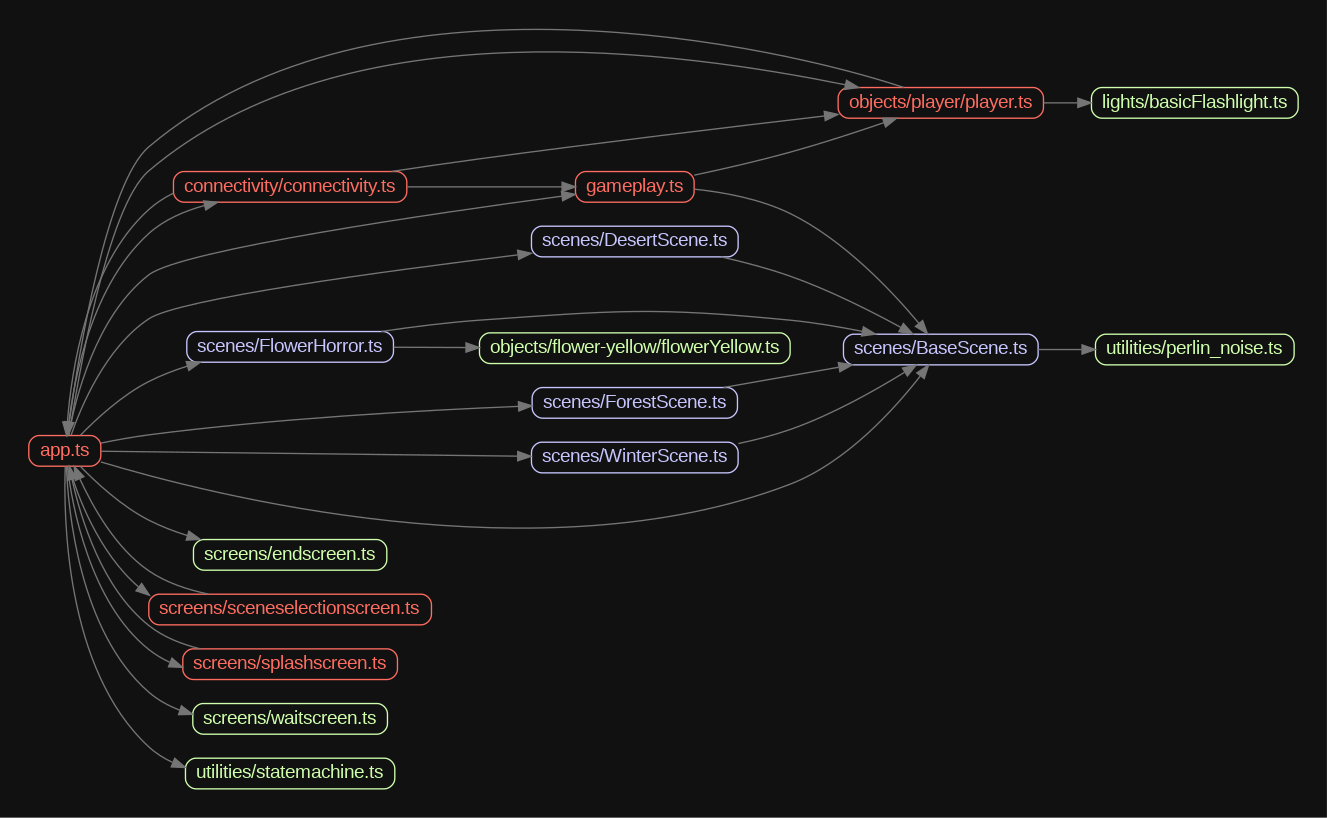
\includegraphics[width=0.7\textwidth]{architecture}
    \caption{Shadow Spy — Software Architecture (generated with madge)}
\end{figure}

\subsection{Minimap}
\par The minimap in the lower-right corner of the game is actually a second 3D render. It shows the camera feed of a second camera that looks down onto the game area. Other than the first-person camera, this is an Orthographic Camera so that we get an undistorted top-view map. Instead of rendering the real player, we represent it through a low-quality sphere.
\par One could argue that rendering a second camera is 'overkill'. But because the camera is only rendering a single sphere with 16 width segments to approximate a circle, the computational effort is negligible.

\subsection{Score Keeping}
\par The player score is updated in a multistep process:
\begin{enumerate}
	\item Compute the distance between both players. If this distance is larger than the flashlight range, we don't have to update the score.
	\item Compute a direction vector that points to the other player and convert it to the local head/camera coordinate system.
		\par Check if the viewing direction and direction to the other player align. Alignment is determined by the flashlight cone angle.
	\item If we still couldn't exclude that we observe the other player, we cast a ray through our scene and look for intersections. If no intersection in the scene is found, we observe the opponent and increase our score. We also of course consider if the flashlight is even turned on.
\end{enumerate}
\par In addition to the true score value, a public score is set. This is only updated when we stop seeing our opponent. This ensures that the other player can't deduce being observed.
\par If one's score exceeds 1000 points, one transitions to the \texttt{SETTLING} state in the state machine to terminate the game and determine the winner.

\subsection{Player Model \& Animations}
\begin{figure}[h] % These figures will appear above the entire subsection, next to each other
    \centering
    \begin{minipage}{0.3\textwidth}
        \centering
        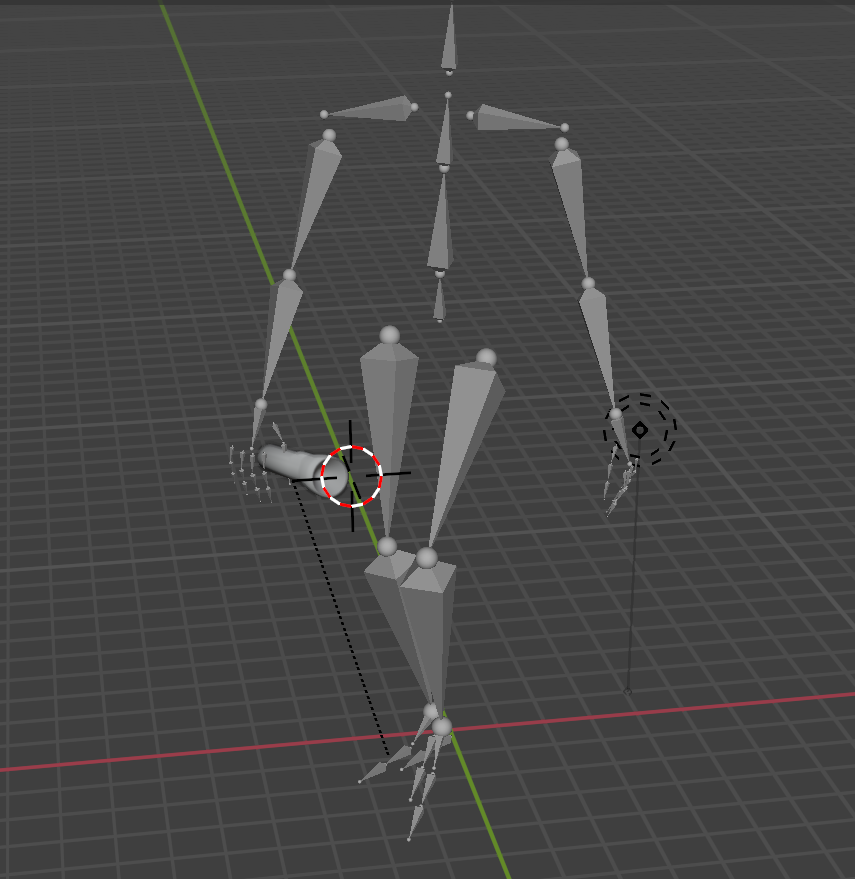
\includegraphics[width=\textwidth]{skeleton}
        \caption{Skeleton with flashlight in Blender}
    \end{minipage}
    \hfill
    \begin{minipage}{0.3\textwidth}
        \centering
        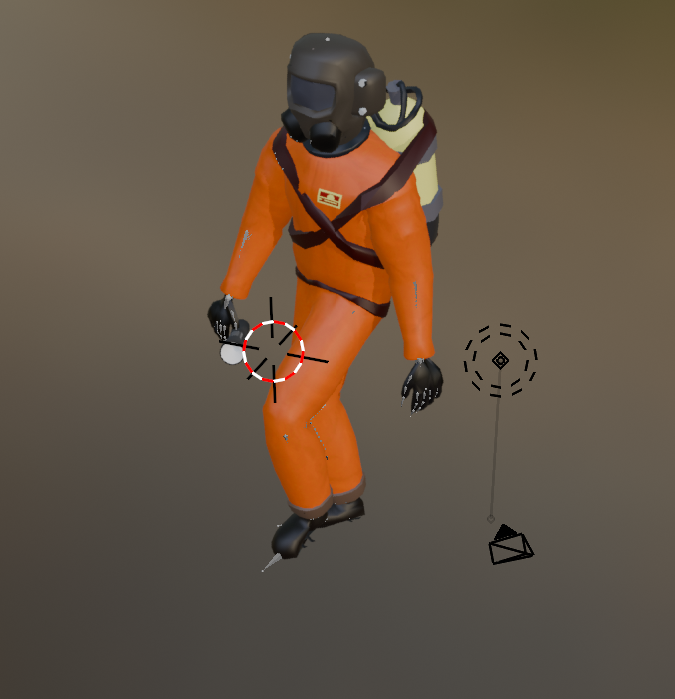
\includegraphics[width=\textwidth]{playerBlender}
        \caption{Full model in Blender}
    \end{minipage}
    \hfill
    \begin{minipage}{0.3\textwidth}
        \centering
        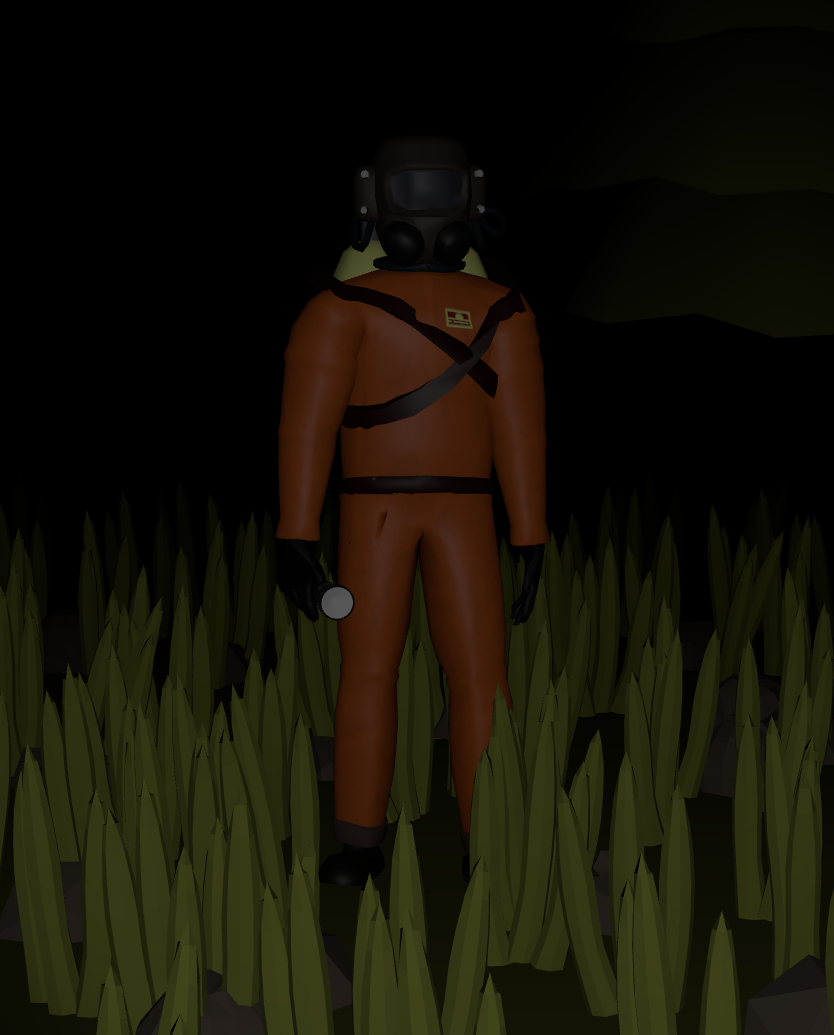
\includegraphics[width=\textwidth]{playerGame}
        \caption{Player model in the game}
    \end{minipage}
\end{figure}


\par This part of the project required a significant amount of time and effort, especially since I had no prior experience with Blender. Conceptually, it involved downloading a player model with an appropriate license and preparing it for use in our game.

\par To achieve this, we matched the model to a skeleton, enabling us to attach animations. Additionally, we attached a separate flashlight model to the player’s hand so that it follows the player’s movements during animations. This step was crucial for gameplay functionality and visual consistency.

\par To integrate animations into our game, we programmed the system to play specific animations corresponding to key presses. Since the animations did not have a consistent base speed, we implemented logic to adjust the playback speed of each animation dynamically. This approach ensured that all animations appeared natural and fluid during gameplay.


\par This part of the project required a significant amount of time and effort, especially since I had no prior experience with Blender. Conceptually, it involved downloading a player model with an appropriate license and preparing it for use in our game.

\par To achieve this, we matched the model to a skeleton, enabling us to attach animations. Additionally, we attached a separate flashlight model to the player’s hand so that it follows the player’s movements during animations. This step was crucial for gameplay functionality and visual consistency.

\par To integrate animations into our game, we programmed the system to play specific animations corresponding to key presses. Since the animations did not have a consistent base speed, we implemented logic to adjust the playback speed of each animation dynamically. This approach ensured that all animations appeared natural and fluid during gameplay.





\par To integrate animations into our game, we programmed the system to play specific animations corresponding to key presses. Since the animations did not have a consistent base speed, we implemented logic to adjust the playback speed of each animation dynamically. This approach ensured that all animations appeared natural and fluid during gameplay.





\subsection{Scenes}
\par There are currently 4 scenes available. (See below Figure 5 -8).

\begin{figure}[h!]
    \centering
    \begin{minipage}{0.3\textwidth}
        \centering
        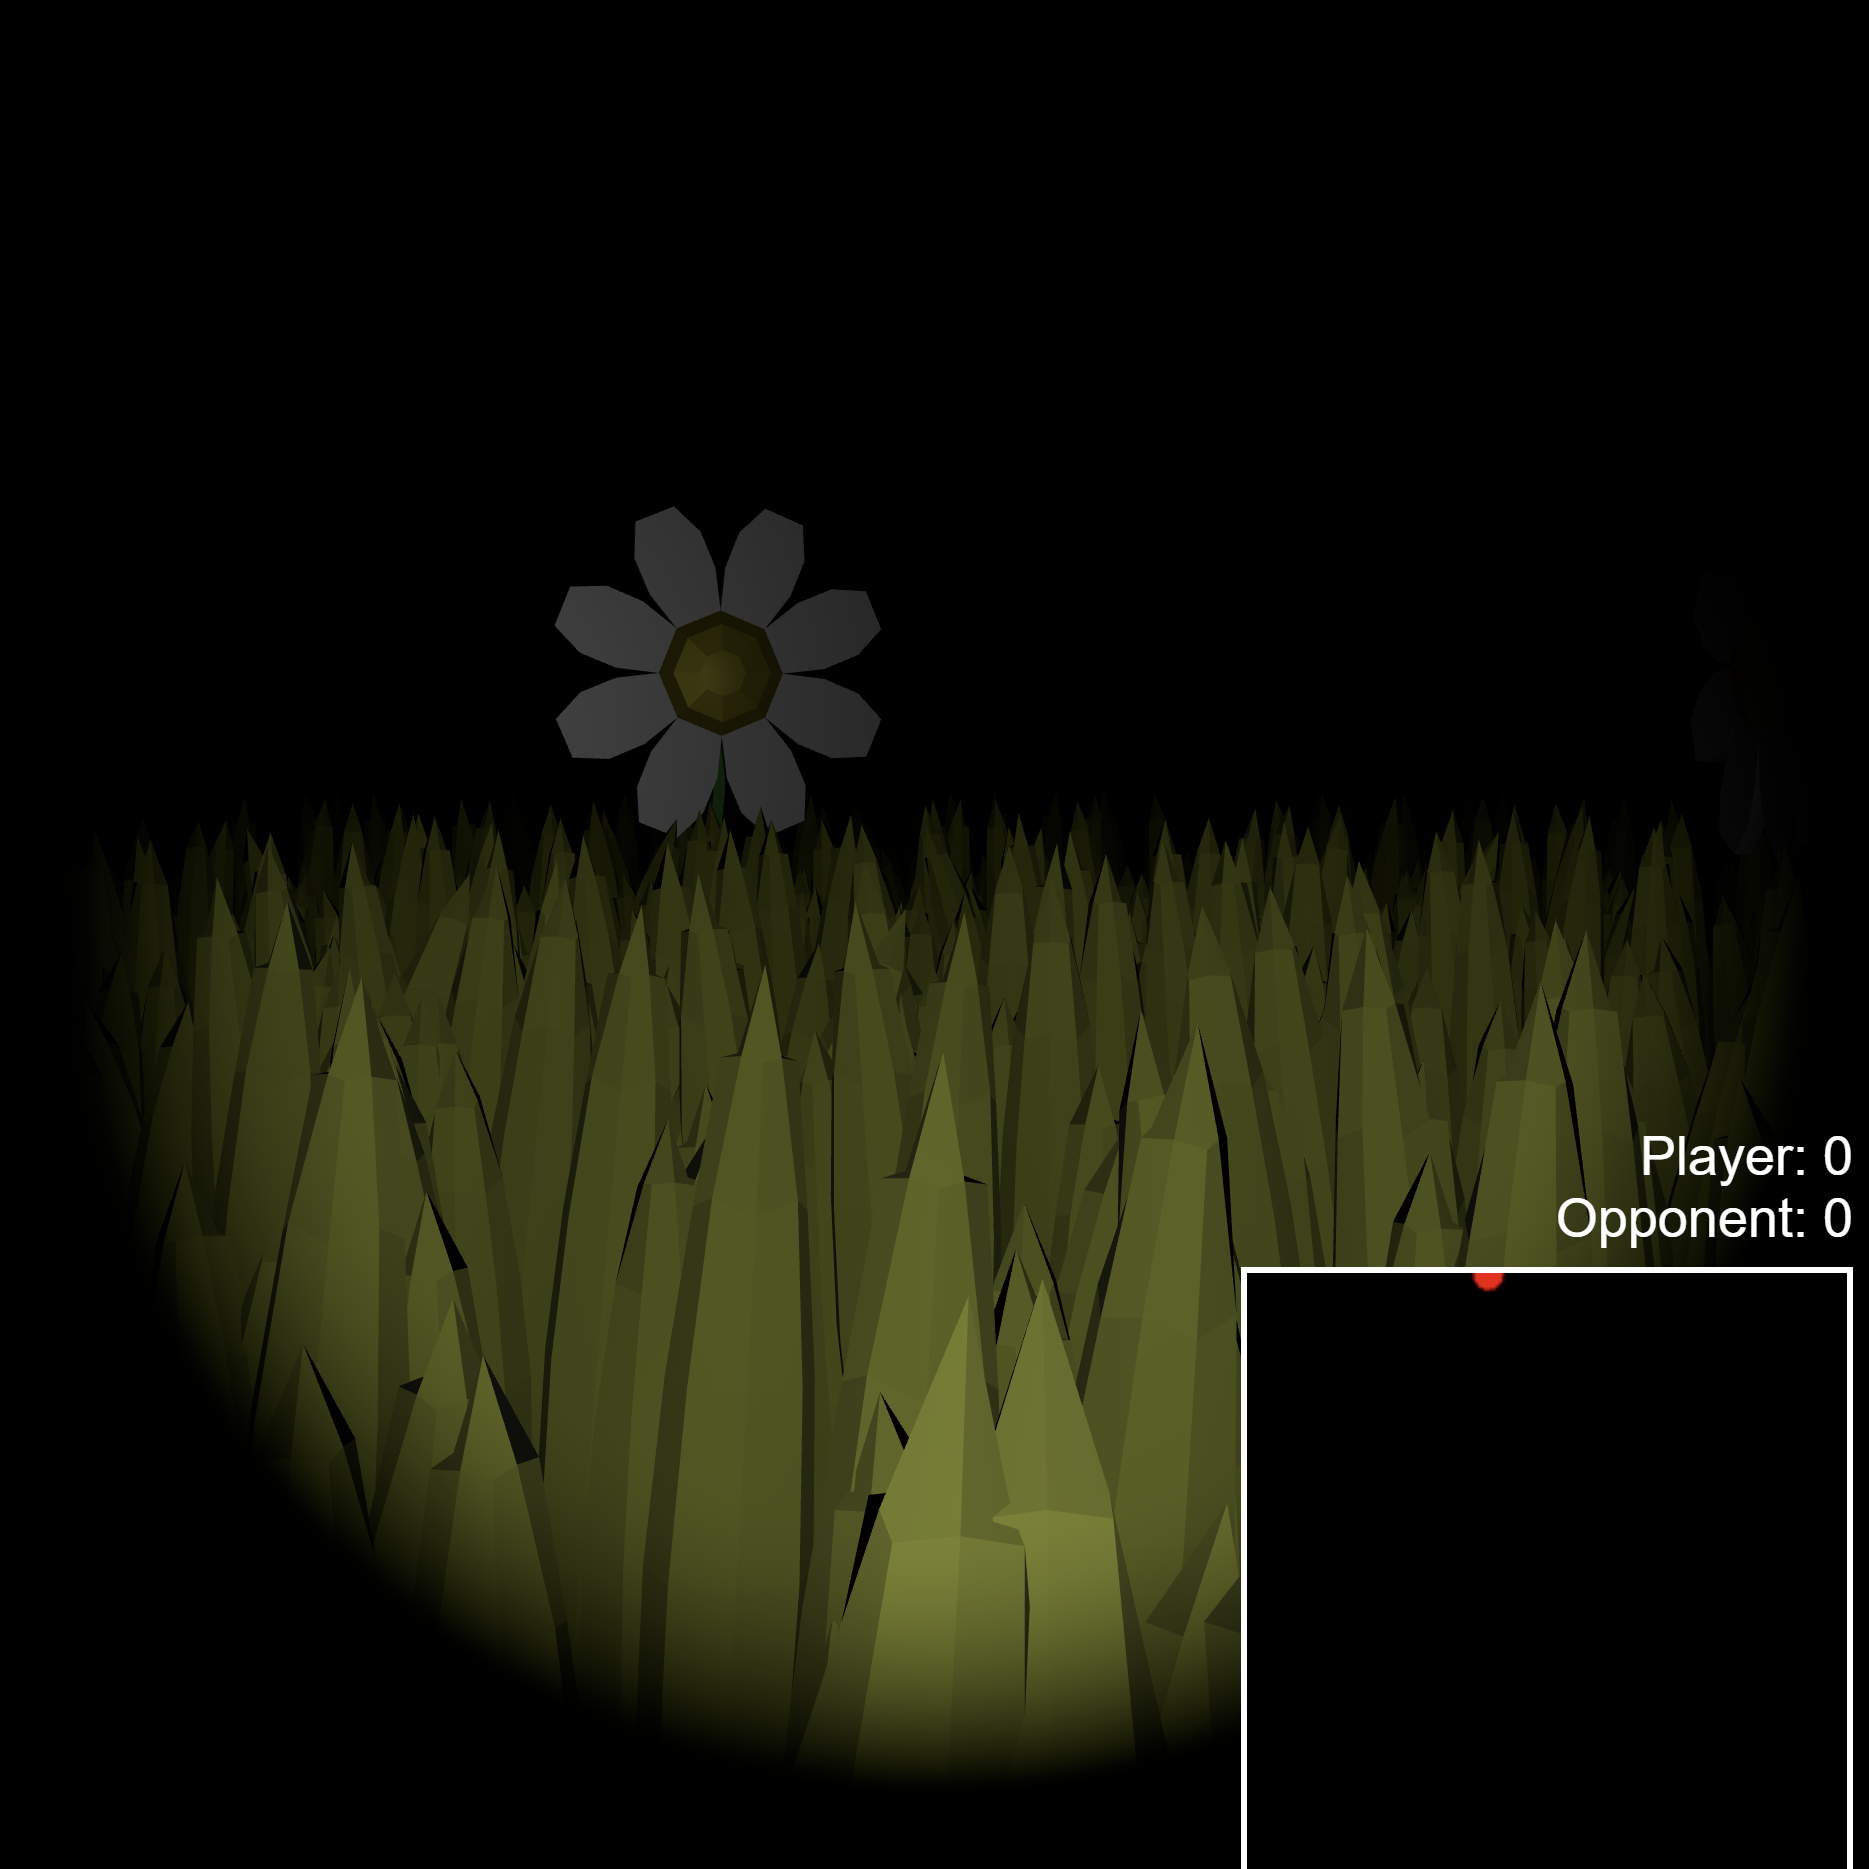
\includegraphics[width=\linewidth]{flowerfield}
        \caption{Flower Horror}
    \end{minipage}%
    \hspace{0.5cm}
    \begin{minipage}{0.3\textwidth}
        \centering
        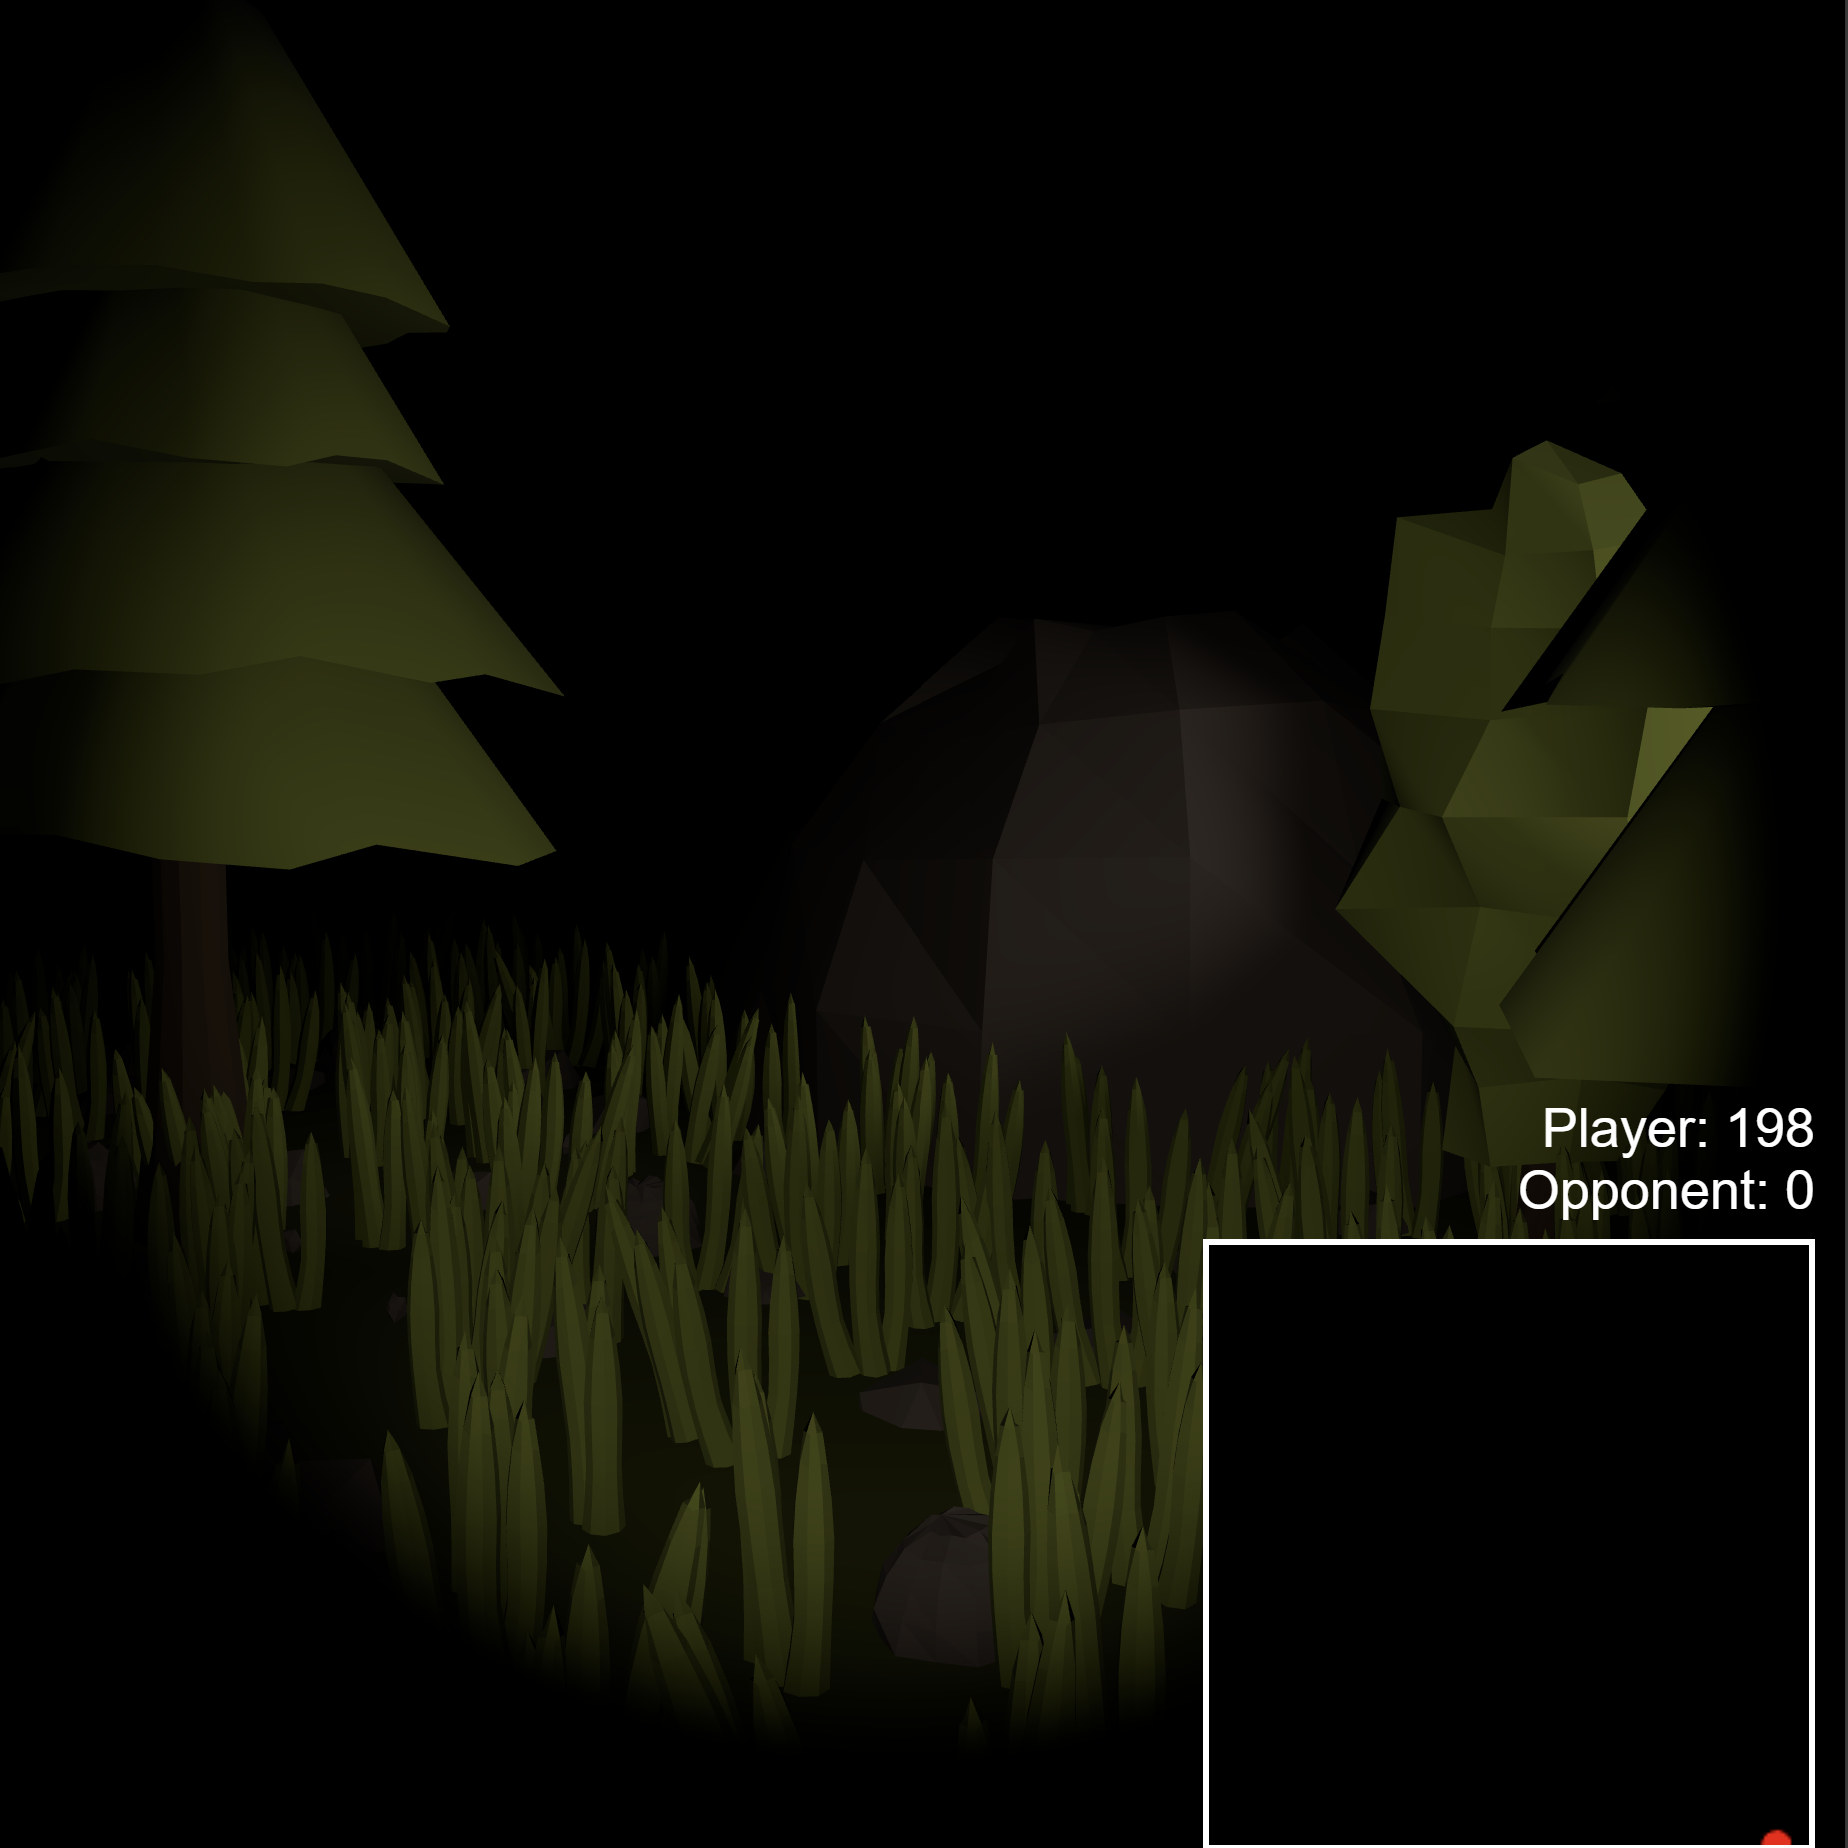
\includegraphics[width=\linewidth]{woodlands}
        \caption{Mixed Woodland}
    \end{minipage}

    \vspace{1cm}

    \begin{minipage}{0.3\textwidth}
        \centering
        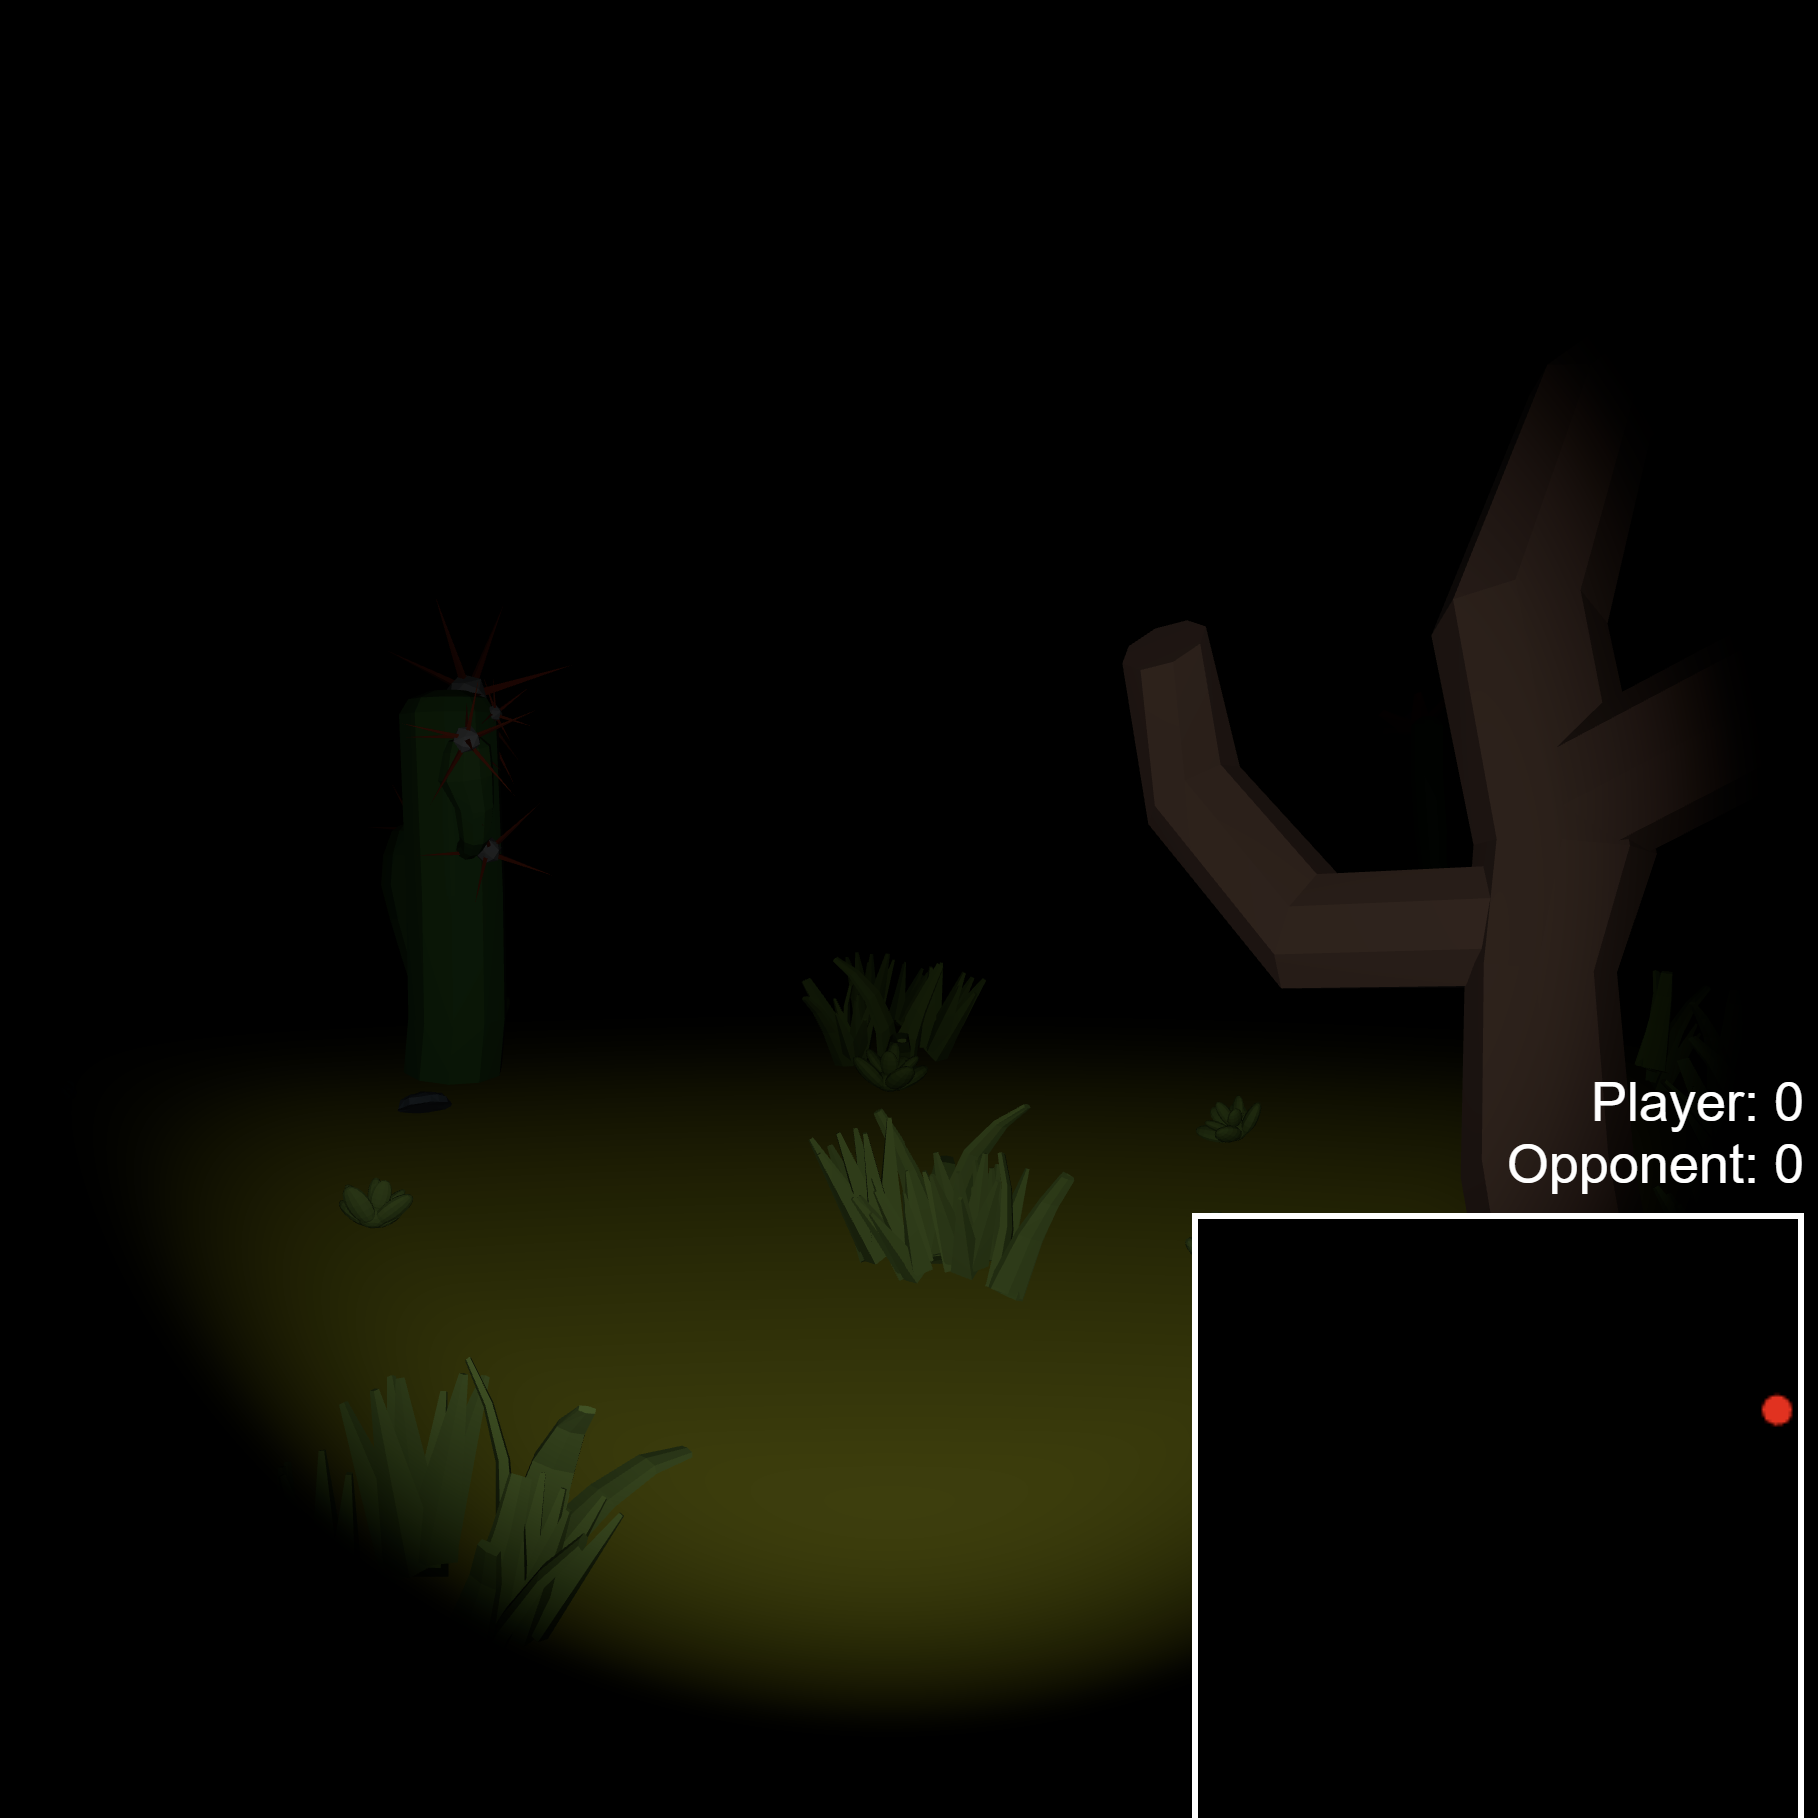
\includegraphics[width=\linewidth]{desert}
        \caption{Desert}
    \end{minipage}%
    \hspace{0.5cm}
    \begin{minipage}{0.3\textwidth}
        \centering
        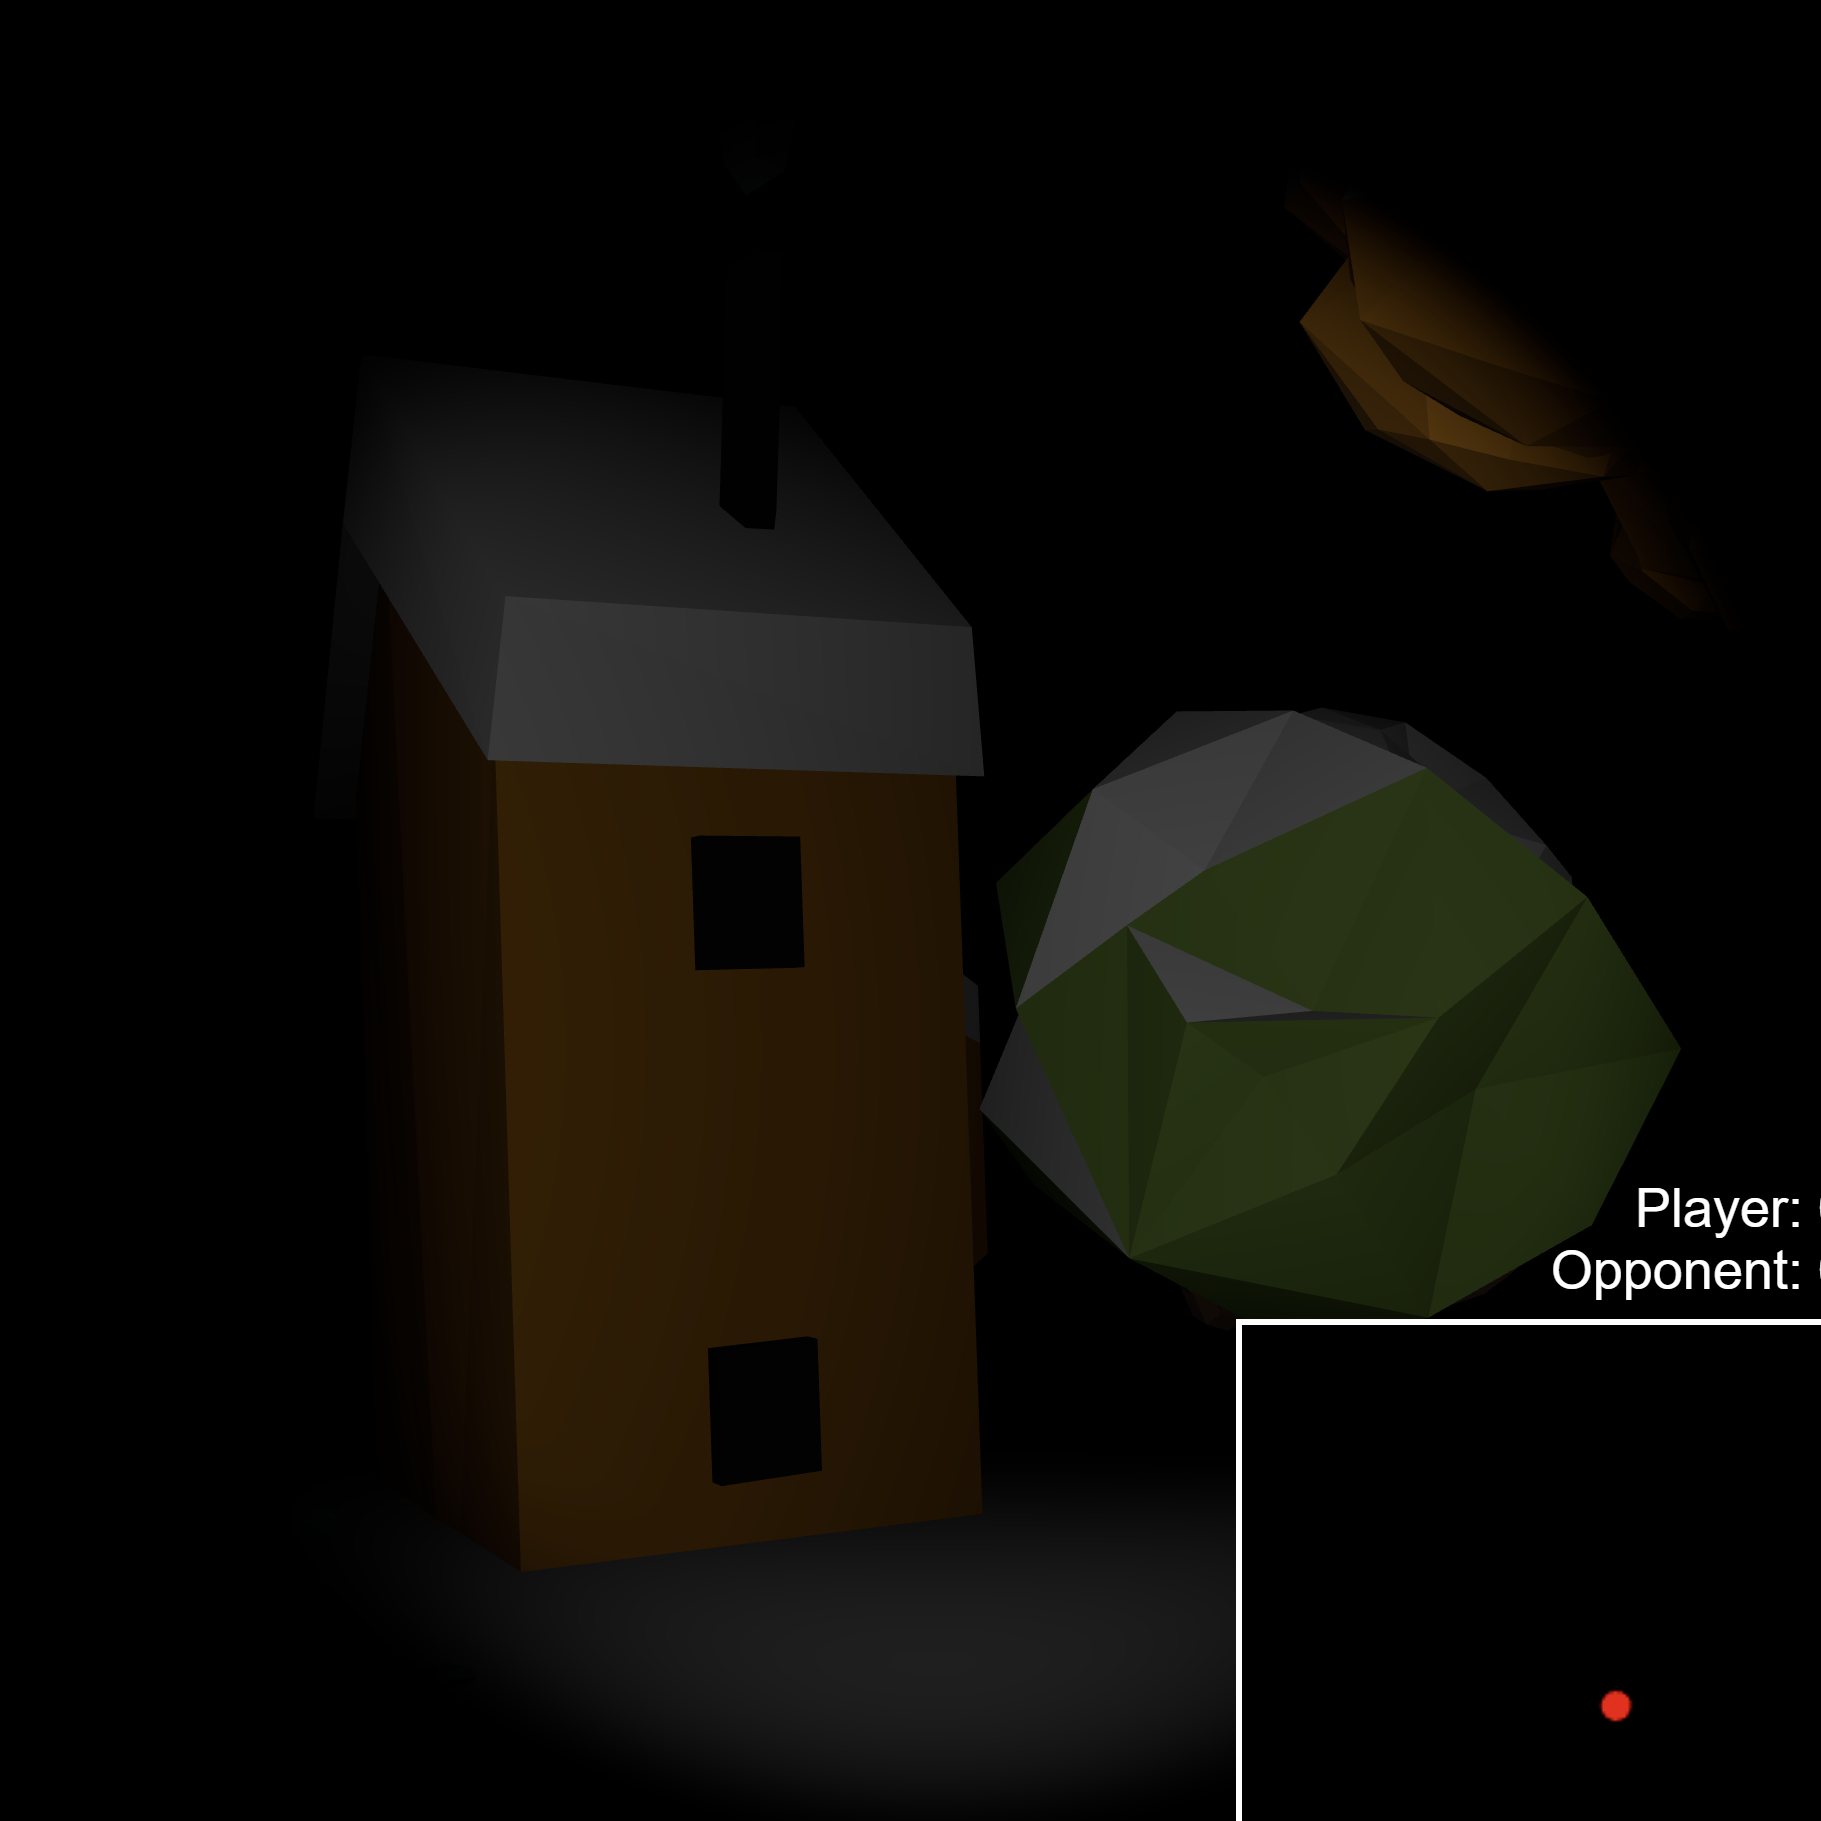
\includegraphics[width=\linewidth]{winter}
        \caption{Winter Village}
    \end{minipage}
\end{figure}

\par All of them are generated roughly in the following way, although the details vary. There is a set of objects that can be generated. From this set, exactly 1 object is generated at each position in a grid over the entire map. 
\par Each object then receives an offset and a rotation to make the scene feel more natural. All of this is randomized and depends on the ID. 
\par Often there are two sets of objects, those with collision (trees, large stones, etc.) and small objects without collision (grass, small stones, and so on) which are generated independently of each other with different frequency.


\subsection{Collision Detection \& Handling}
\par Collision detection is basic right now, all objects which have collision, simply are represented as a bounding box. To check if two objects collide, one tests if those two boxes intersect.
\par Additionally, some objects have a manually downsized collision box because it felt more accurate/smoother to play this way. 
\subsection{Audio}

% ASPECTS
% - choices
% - approaches
% - implementation hurdles
% - features implemented
% - diagrams of project architecture




% -----------------------------------------------------------------

\section{Results}
\par The final game provides a simple user experience. The game can be played by running the JavaScript application locally or visiting \href{https://google.com}{https://roldsi.github.io/shadow-spy/}. It is also possible for one player to use the locally deployed version and the other player to use the web-version.
\par To initiate a game, one player 'Player A' and the other player chooses 'Player B' on the splashscreen. Player A enters the code shown to player B. This establishes the connection between both browsers. Player A can then configure the game by choosing a scene.
\par As soon as player A chooses a scene, the game starts for both players. The user is placed at a random position in the world, sufficiently far away from the other player. Depending on the browser, it may be necessary to click onto the browser window once to activate first-person controls. One can walk with the keys 'wsad', rotate by moving the cursor and turn the flashlight on /off with 'f'. There is also background music.
\par On the bottom right, the player can see a mini-map of the world with its position. Above, one can see one's own count and the other player's count. One gains points whenever one sees one's opponent. Peeking from behind an object at the opponent only counts when a sufficiently clear line of sight exists.
\par If one is observed by the opponent, one doesn't see the opponent score increase immediately. Their gains will only be shown once one is no longer observed to avoid using the score counter as an indicator of the presence of the opponent.
\par If both players observe each other, they are repositioned to new random locations in the map to avoid a stalemate.
\par The first player to reach 1000 points wins the game. As soon as that happens, the game is terminated for both players.





% -----------------------------------------------------------------

\section{Discussion}
\par Any project can be improved arbitrarily. At this point, we are not aware of any big issues or bugs with the game, but have various ideas for additional features or possible improvements.
\par We only list a selection of our ideas here to keep the report reasonably short.

\subsection{Pairing \& Scaling}
\par Initially, the pairing process required that player A enters a long randomized string provided by the pairing server because every active connection with the pairing server must have a unique ID. We avoid manually typing a long random string, we generate a short player code and appending a long game-specific string. This string is likely to be unique, but that is not guaranteed.
\par If the game were played by hundreds of people simultaneously, it will be likely that the same ID is used by multiple players. The game synchronization will break in that case.
\par A solution would be a more advanced pairing and discovery protocol. Considering that his is a graphics project at the core, this was out of scope.

\subsection{Customization}
\par Player A can choose from a limited set of scenes at the beginning of the game. One could add more different scenes and improve the degree of randomization within those scenes.
\par Additionally, one could provide the user with more customization options, such as different characters or flashlights to choose from.

\subsection{Lighting}
\par Given the pre-defined player model with its flashlight, there is currently limited variety in scene lighting. The game could become more interesting by adding choices between different types of flashlights: Long-range but narrow, wide but short-range, … Having a brighter flashlight is not necessarily an advantage because one can be tracked easier.
\par Besides basic flashlights, one could also introduce power-ups that can be gained throughout the game. For instance, a player could gain night vision for a limited time. This would give a one-sided advantage.
\par An even other option to introduce variety would be the weather. Rain and fog could make visibility more difficult. While lightning could add bright momentary global illumination.




% -----------------------------------------------------------------

\section{Ethical Evaluation}
\subsection{Copyright}
We ensured that all materials used in our project, which were mostly 3D Models and audio, were properly licensed, aligning with the ACM Code of Ethics and Professional Conduct. This also matches with Principle 1.3: Be honest and trustworthy and Principle 1.6: Respect privacy and confidentiality. By sourcing content only from reputable, license-compliant platforms and verifying permissions for third-party assets, we maintained transparency and avoided misappropriation of intellectual property. This approach not only upholds legal standards but also respects the labor and creativity of original creators.

Additionally, our process demonstrates Principle 2.5: Give proper credit for intellectual property. We provide clear attribution when required (namely in the Credits Section below), recognizing the contributions of others. This ethical stance promotes fairness, encourages innovation, and reduces legal risk.

\subsection{Representation}
Recognizing the importance of character selection in games, we initially aimed to include this feature. However, due to limited animation experience and a tight development timeline, we determined that a fully customizable system was beyond our scope. This challenge prompted reflection on how to approach character design ethically and inclusively.

We aligned our approach with the ACM Code of Ethics and Professional Conduct, particularly Principle 1.4: Be fair and take action not to discriminate and Principle 1.2: Avoid harm. Our goal was to ensure the character model would be relatable, respectful, and free from harmful stereotypes.

After discussion and research, we selected an "astronaut"-style model that met these criteria. Its non-sexualized design avoided over-sexualization, a prevalent issue in character representation. Moreover, its fully enclosed suit and helmet obscured race, gender, and other identifiers, allowing for broader representation. This choice enabled a diverse range of players to see themselves reflected in the character.


\section{Contribution}
Flurin did most of the modeling, animations, scenes. Simon did the networking, controls. code skeleton, scoring, lighting, prototype.


% -----------------------------------------------------------------

\section{Resources/Credits}
\begin{itemize}
	\item Three.JS
	\item Player model : This work is based on "Lethal Company Scanvenger (Player Model) Rigged" (https://sketchfab.com/3d-models/lethal-company-scanvenger-player-model-rigged-465a867f402f46bcb6fe2d8848941829) by BenjiSkye15 \newline (https://sketchfab.com/BenjiSkye15) licensed under CC-BY-4.0 \newline (\http://creativecommons.org/licenses/by/4.0/)
	\item Assets (mainly for Woodlands but also for Flower) : Trees & Rocks by Sham Al Bdour [CC-BY] via Poly Pizza 
	\item Assets for Desert :  \newlineWild West Scene by Jacques Fourie [CC-BY]  via Poly Pizza 
	\item Assets for Winter :  Winter in the Hinterland by Matt Connors [CC-BY] Poly Pizza 
\end{itemize}


% -----------------------------------------------------------------




\end{document}
